\documentclass[a4paper, 12pt]{book}
\usepackage[utf8]{inputenc}
\usepackage[T1]{fontenc}
\usepackage[frenchb]{babel}
\addto\captionsfrench{\def\tablename{Tableau}}
\usepackage{float}
\usepackage{multirow}
\usepackage[table]{xcolor}
\usepackage{lmodern}
\usepackage{ae,aecompl}
\usepackage[top=2.5cm, bottom=2cm, 
			left=3cm, right=2.5cm,
			headheight=15pt]{geometry}
\usepackage{graphicx}
\usepackage{pgfplots}
\pgfplotsset{compat=1.14}
\usepackage{eso-pic}
\usepackage{array}
\usepackage[colorinlistoftodos]{todonotes}
\usepackage[colorlinks=true, allcolors=blue]{hyperref}
\makeatletter
\def\@ecole{école}
\newcommand{\ecole}[1]{
  \def\@ecole{#1}
}
\def\@domaine{}
\newcommand{\domaine}[1]{
  \def\@domaine{#1}
}

\def\@specialite{Spécialité}
\newcommand{\specialite}[1]{
  \def\@specialite{#1}
}


\def\@master{Master}
\newcommand{\master}[1]{
  \def\@master{#1}
}

\def\@adresse{Adresse}
\newcommand{\adresse}[1]{
  \def\@adresse{#1}
}

\def\@encadranta{}
\newcommand{\encadranta}[1]{
  \def\@encadranta{#1}
}

\def\@encadrantb{}
\newcommand{\encadrantb}[1]{
  \def\@encadrantb{#1}
}
\def\@auteura{}{}{}
\newcommand{\auteura}[1]{
  \def\@auteura{#1}
}
\def\@auteurb{}{}{}
\newcommand{\auteurb}[1]{
  \def\@auteurb{#1}
}
\def\@auteurc{}{}{}
\newcommand{\auteurc}[1]{
  \def\@auteurc{#1}
}
\def\@auteurd{}{}{}
\newcommand{\auteurd}[1]{
  \def\@auteurd{#1}
}
\makeatother




\makeatletter
\newcommand{\pagedegarde}{
\newgeometry{top=2.5cm, bottom=1cm, left=2cm, right=1cm}
  \begin{titlepage}
  \centering
      
\includegraphics[width=1\textwidth]{limogelogo.pdf}
    \vspace{1cm}
      {\huge 
    \vspace{0.5cm}
        {\huge\bfseries \@ecole}\\
    \vspace{0.2cm}
        {\Large\bfseries \@domaine}\\
    \vspace{0.5cm}
        {\Large\bfseries Master 1 }\\
    \vspace{0.2cm}
        {\large\bfseries Sécurité informatique et cryptologie }\\
    \vspace{1cm}
    	MEMOIRE DU SECOND SEMESTRE}\\
    \vfill
       {\LARGE \color[rgb]{0,0,1} \bfseries{\@title}} \\
    \vspace{2cm}
    	{\bfseries \@auteura}\\
    	{\bfseries \@auteurb}\\
    	{\bfseries \@auteurc}\\
    	{\bfseries \@auteurd}\\
    \vspace{0.5cm}
        Encadrants :\\
        {\bfseries \@encadranta}\\
        {\bfseries \@encadrantb}\\
    \vspace{0.5cm}
        {\Large\bfseries \@date}\\
    \vfill
  \end{titlepage}
\restoregeometry
}
\author{}
\auteura{Thanina \textsc{Alili}}
\auteurb{Thibault \textsc{Debonnière}}
\auteurc{Baptiste \textsc{Decrand}}
\auteurd{Ndiasse \textsc{Thioune}}
\title{Analyse Forensic d'un Ransomware}
\master{Master 1 Informatique}
\specialite{CRYPTIS}
\encadranta{Jean-Louis \textsc{Lanet}}
\encadrantb{Benoit \textsc{Crepin}}
\date{20 avril 2018}
\ecole{UNIVERSIT\'{E} DE LIMOGES}
\domaine{
	\textbf{FACULT\'{E} DES SCIENCES ET TECHNIQUES}
}
\begin{document}
\pagedegarde
\newpage
\pagebreak
\hspace{0pt}
\vfill
\section*{Remerciements}
\paragraph{}
Nous souhaitons remercier notre encadrant M. Jean-Louis  LANET, professeur des Universités et directeur du laboratoire de haute sécurité de Inria-Rennes-Bretagne-Atlantique pour nous avoir confié ce sujet, pour le temps et les connaissances qu'il nous a apportées afin que le projet se déroule dans les meilleures conditions possibles.
Nous remercions également M. Benoît CRESPIN, Maître de conférence et responsable des projets informatiques en master pour son organisation et le temps qu'il a dédié à l'encadrement des étudiants.
\vfill
\hspace{0pt}
\tableofcontents
\listoffigures
\listoftables
\chapter*{Introduction}
\addcontentsline{toc}{chapter}{Introduction}
  \todo[inline, color=green!40]{Introduction non fini}
\paragraph{}
    Ce rapport est une suite du travail effectué durant le premier semestre qui vient concrétiser les recherches et la partie théorique mais également le prototypage mis en place, en une application capable d'analyser les ransomwares selon des critères bien définis.
\paragraph{}
    Un ransomware est un malware qui peut restreindre ou empêcher l'accès système en cryptant les fichiers ou juste en verrouillant l'écran système de façon à forcer l'utilisateur à payer une rançon. Ces attaques ont fait leurs preuves en extorquant des sommes d'argent considérables. Actuellement, ces ransomware modernes sont regroupés en tant que crypto-ransomware qui chiffrent certains types de fichiers systèmes infectés et obligent l'utilisateur à payer une rançon avec un paiement en ligne afin d'obtenir une clé de décryptage. Il existe différentes manières de propagation de ransomware, principalement les sites web, e-mails et fichiers partagés.
\paragraph{}
	Le premier malware de ce type est identifié en 1998 avec pour nom de code "PC Cyborg". Il utilisait un cryptage symétrique simple,il était donc facile de mettre en place des outils pour décrypter les fichiers cryptés par PC Cyborg. En 2012, le fait de tenir les machines des utilisateurs pour les paiements de rançons est devenu très courant avec l'arrivée du malware Reveton. Ce dernier empêche tout utilisateur d'accéder à son ordinateur sauf s'il accepte de payer une rançon en passant par un service de paiement tel qu'Ukash Bitcoin. Deux ans plus tard, CryptoLocker apparut. Son but est de chiffrer les fichiers des utilisateurs et d'exiger une rançon pour les décrypter. Il devient le modèle de la plupart des types de ransomware apparu depuis. On répertorie deux principaux ransomwares: Locker ransomware, qui verrouille l'appareil, et Crypto ransomware qui empêche l'accès aux données souvent par cryptage.
    \todo[inline, color=green!40]{Remarques BD: - Il faudrait maintenant poser le problème et expliquer le projet}
\paragraph{}
\todo[inline, color=green!40]{Remarques BD: - il faudrait ajouter une présentation sur Inria-RBA et l'utilisation de la base de donnée dans le projet}
	Dans une première partie du rapport, nous abordons l'implémentation de l'application avec les vecteurs, les métriques utilisées et les fonctionnalités existantes et apportées. En seconde partie on retrouve tout ce qui se rapporte à la qualité et la performance de l'application ainsi que les tests réalisés. Enfin nous terminons par dresser un bilan global de notre travail sur ce projet.
    
   
 	 
    

\newpage
\chapter{Implémentation de l'application}
\newpage
\section{Construction des vecteurs}
L'application a pour principale fonctionnalité de reconnaître et de classifier des ransomwares en analysant des captures mémoires de programmes. Les captures mémoires contiennent des chaînes de caractères correspondant à des appels systèmes ou à des librairies qui caractérisent le processus lancé. Notre application va récupérer ces chaînes de caractères  sous la forme de vecteur binaire et les comparer à d'autres afin de déduire à quelle sorte de programme appartient la capture mémoire étudié. L'application va donc transformer la capture mémoire étudiée en vecteur binaire et calculer la similarité de ce vecteur avec des vecteurs caractérisants différentes familles de ransomwares. De ce calcul, l'application déduit et informe l'utilisateur de quelle famille le programme étudié ressemble le plus. Les vecteurs qui caractérise les familles de ransomware seront appelés vecteurs familiaux, le vecteur qui est généré depuis une capture mémoire soumis par l'utilisateur sera nommé vecteur sujet. Ces vecteurs sont binaire, de même dimension et chacune de leurs composantes représente un terme spécifique tel qu'un appel système ou une librairie sont basé sur un vecteur dit modèle. Une composante dont la valeur est 1 signifie que le terme associé est contenu, la valeur 0 indique que le terme n'est pas contenu. 
\paragraph{}
Les vecteurs familiaux et le vecteur modèle sont construits en se basant sur la base de données de Inria-RBA. Cette base de donnée contient des dumps mémoire de ransomware qui sont déjà classifiés. Les vecteurs familiaux et le vecteur modèle sont enregistrés dans des fichiers de données que l'application va récupérer lors de son initialisation.
\subsection{Vecteur modèle}
Le vecteur modèle va servir de patron à l'ensemble des vecteurs binaires, comme il définit la structure des vecteurs binaires que l'application va construire, utilisé ou comparé, le vecteur modèle sera le premier à être instancié par l'application, celui-ci va lire un fichier de donnée (prenant la forme d'un dictionnaire) contenant l'ensemble des termes qui permettent de caractériser des ransomwares.
\paragraph{}
Les caractéristiques des vecteurs binaires seront établies par ce dictionnaire. La première composante du vecteur binaire correspondra au premier terme du dictionnaire, la deuxième composante au second terme etc. la dimension N d'un vecteur binaire est la taille de ce dictionnaire. Pour le vecteur modèle, chaque composante sera initialisé à 0 (ce qui signifie faux ou non contenu), ce choix permettra de générer les vecteurs familiaux et les vecteurs sujets. En effet chaque fois que l'application aura besoin de construire un nouveau vecteur, elle utilisera le vecteur modèle comme vecteur initial puis les valeurs des composantes qu'elle estimera à 1 (ce qui signifie contenu). On peut voir dans la figure~\ref{vecteurmodele} la forme d'un vecteur modèle.
\paragraph{}
\begin{table}[h]
  \centering
\begin{tabular}{|c|c|c|}
    \hline
    \rowcolor{gray}
   N\degre\space Composant& Termes & Valeurs\\
    \hline 
       0&ADVAPI32.dll&0\\
    \hline 
       1&lstrcpynA&0\\
    \hline
       2&RtlFreeUnicodeString&0\\
    \hline 
       ...&...&0\\
    \hline 
       N-1&NetApiBufferFree&0\\
    \hline
       N&SearchPathW&0\\
    \hline
\end{tabular}\\
\caption{Structure du vecteur modèle}
\label{vecteurmodele}
\end{table}
\newpage
\subsection{Vecteurs familiaux}
\paragraph{}
Un vecteur familial représente une famille de ransomware spécifique, il est basé sur le vecteur modèle, cependant l'ensemble des composantes correspondant aux termes caractérisant sa famille ont pour valeur 1 (contenu). En calculant la distance de ces vecteurs au vecteur du fichier que l'utilisateur souhaite étudier l'application va pouvoir établir à quel ransomware il correspond le mieux.
\paragraph{}
Les vecteurs familiaux sont créés au sein de l'application après le vecteur modèle, ceux-ci sont dans un premier temps instanciés comme une copie du vecteur modèle puis chaque vecteur va se baser sur un fichier de données qui lui est spécifique et qui contient une liste des termes caractérisant sa famille, il va alors modifier les valeurs des composantes correspondant à ces termes à 1 (contenu). On peut voir dans le tableau~\ref{VecteurFamiliale} la forme d'un vecteur modèle.
\paragraph{}
\paragraph{}
\begin{table}[h]
  \centering
\begin{tabular}{|c|c|c|}
    \hline
    \rowcolor{gray}
   N\degre\space Composant& Termes & Valeurs\\
    \hline 
       0&ADVAPI32.dll&0\\
    \hline 
       1&lstrcpynA&1\\
    \hline
       2&RtlFreeUnicodeString&1\\
    \hline 
       ...&...&...\\
    \hline 
       N-1&NetApiBufferFree&1\\
    \hline
       N&SearchPathW&0\\
    \hline
\end{tabular}\\
\caption{Structure d'un vecteur familial}
\label{VecteurFamiliale}
\end{table}
\paragraph{}
Les fichiers de données permettant d'instancier les vecteurs familiaux ont été établis avec la base d'apprentissage de Inria-RBA, celle-ci contient pour chaque familles de ransomware un ensemble de fichiers de captures mémoires de l’exécution de ces ransomwares.
\paragraph{}
Pour établir la liste des termes caractéristique d'une famille de ransomware, on extrait les termes que l'on retrouve en majorité dans les fichiers de captures de mémoire de ce type de ransomware, afin de connaître le meilleur taux correspondant à cette majorité, nous avons comparé la qualité de détection de l'application avec différents taux en utilisant le base de données test de Inria-RBA.

\begin{figure}[!h]
\centering{
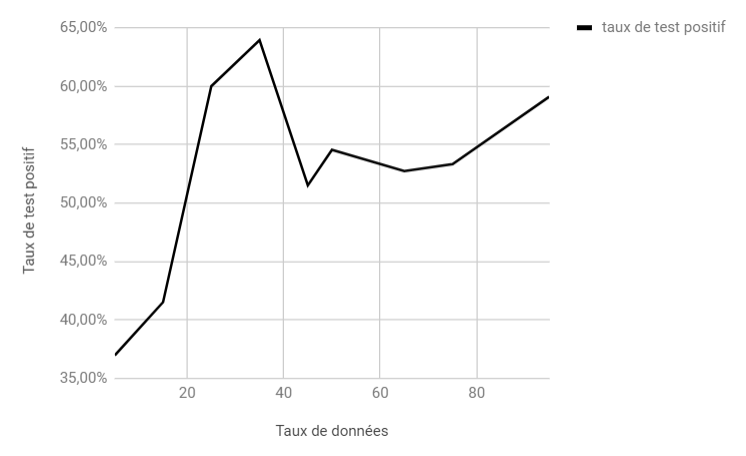
\includegraphics{Taux.PNG}}
\caption{Taux de test positif en fonction de la majorité de terme conservés}
\label{graphTaux}
\end{figure}
\newpage
\paragraph{}
On remarque à travers le graphique de la figure~\ref{graphTaux}, que le taux de réussite est le plus élevé quand on utilise 35 \% des données les plus communes, cela signifie que 35\% des termes les plus présents représente au mieux la famille du ransomware et peuvent être considéré comme des termes caractéristiques de cette famille.
Grâce à la base de donnée de Inria-RBA, nous avons pu généré plusieurs vecteurs familiaux dont voici la liste:
\begin{itemize}
\item bitman
\item cerber
\item deshacop
\item fsysna
\item gamarue
\item telsacrypt
\item xorist
\item yakes
\item zerber
\item goodware
\end{itemize}

L'application a la possibilité de détecter ces neufs familles de ransomware, la famille goodware correspond aux logiciels sans intentions malveillantes et permettra de distinguer les ransomwares des autres logiciels.

Le vecteur modèle a une dimension d'environ deux milles termes et chaque familles contient environ deux cents termes caractéristiques. Certains de ces termes pouvant se retrouver dans plusieurs familles.  
\section{Implémentation des métriques}
\paragraph{}
Une fois que l'application a terminé son initialisation et a réussi à générer le vecteur modèle et les vecteurs familiaux, l'utilisateur va pouvoir analyser un ou plusieurs fichiers.
\subsection{Extraction et construction du vecteur sujet}
\paragraph{}
	L'analyse des données d'un fichier mémoire débute par l'extraction des chaînes de caractères, de la même manière que la commande UNIX "strings", l'extracteur va parcourir une fois le fichier et extraire les termes qui permettent de caractériser les ransomwares et construire un vecteur binaire du fichier étudié à l'aide du vecteur modèle. C'est le vecteur sujet.
\paragraph{}
Ce vecteur sujet est initialisé avant l'extraction comme une copie du vecteur modèle avec l'ensemble de ces composants à 0, pendant l'extraction, à chaque fois qu'un terme est trouvé, le composant correspondant au terme est mis à 1, A la fin de l'extraction le vecteur sujet a l'ensemble de ces composants à 0 pour les termes non contenus dans le fichier et 1 pour les termes contenus.
\paragraph{}
Pour récupérer les termes, l'extracteur va lire le fichier ligne par ligne et découper chaque ligne en liste de mots sachant que les caractères de séparation est l'ensemble des caractères non contenu dans les chaînes de caractères qui nous intéresse c'est à dire tout les caractères autres que l'alphabet,les nombres et quelques caractères (point, underscore...). L'outil va ensuite appliquer des filtres afin d'optimiser l'extraction et éviter ainsi de parcourir le vecteur modèle pour chaque mot. Afin de rendre l'extraction la plus efficace possible, les filtres sont présenté de la plus sélective à la moins sélective.
\paragraph{}
Un premier filtre retiendra les mots de taille raisonnable (entre quatre et trente caractères) puis des filtres retiendront les termes  dont la structure orthographique correspondant à des appels systèmes et à des fichiers de librairies ( La structure orthographique des appels systèmes suit le modèle "Camel Case" tandis que les noms de fichiers de librairies finissent par ".dll". )
\paragraph{}
Lorsque qu'un mot passe les filtres, l'extracteur regarde si ce mot correspond à un terme du vecteur modèle et si c'est le cas, il indique dans le vecteur sujet que le terme est contenu.L'algorithme parcours le vecteur modèle de manière dichotomique  afin d'optimiser la recherche des termes.

Une fois le fichier parcouru, le vecteur sujet est totalement généré. Il suffit ensuite de le comparer aux vecteurs familiaux afin d'obtenir les résultats.
\newpage
\subsection{Calcul des distances vectoriels}
\paragraph{}
Le calcul des distances vectoriels compare chaque vecteurs familiaux avec le vecteur sujet construit par l'extraction. Pour obtenir la distance entre deux vecteur, l'algorithme va dans un premier temps parcourir les deux
vecteurs et calculer la somme des quatre différentes possibilités:
\begin{itemize}
\item Cas $0_{sujet}0_{familial}$ Le terme n'est pas contenu dans le vecteur sujet et le vecteur familiale 
\item Cas $1_{sujet}0_{familial}$ Le terme est uniquement contenu dans le vecteur sujet
\item Cas $0_{sujet}1_{familial}$ Le terme est uniquement contenu dans le vecteur familiale
\item Cas $1_{sujet}1_{familial}$ Le terme est contenu dans les deux vecteurs
\end{itemize}
Une fois ces données obtenus, il suffit d'appliquer la formule de la métrique que l'on souhaite associer.
Par exemple pour la métrique d'Anderberg on réalise la division:
\newline
\begin{equation}
   Distance = \frac{S1_{sujet}1_{familial}}{S1_{sujet}1_{familial} + 2\times(S1_{sujet}0_{familial}+S0_{sujet}1_{familial})}
\end{equation}
\newline
L'algorithme n'a plus qu'à appliquer les calculs de chaque métrique souhaitée, l'ensemble de ces métriques est détaillés dans le premier rapport.
Au niveau de l'application, comme la première partie est commune à toutes les métriques, il a été implémenté une classe "Métrique"  qui est abstraite, celle-ci défini les quatre variables qui contiennent la somme de chaque possibilités et la fonction de l'algorithme qui consiste à parcourir les deux vecteurs et à calculer ces variables. Chaque métrique a sa classe héritant de la classe "Métrique" et définis leurs propres fonctions de calcul.
Cela permet d'éviter de parcourir plusieurs fois les deux vecteurs si l'utilisateur souhaite utiliser différentes métriques.
\paragraph{}

\section{Fonctionnalités}
\todo[inline, color=red!40]{Remarques BD: - Faire cette partie d'Urgence}
    % * <baptistedecrand@gmail.com> 2018-04-10T13:14:13.026Z:
% 
% Dans cette partie, on doit pouvoir retrouver la liste des fonctionnalités de l'application: 
% - Detecter les ransomwares (avec les métriques disponibles, les familles de ransomwares possibles...)
% - La gestion d'erreur
% - L'interface graphique (partie Ndiasse)
% - La detection des clefs (partie thanina)
% - ...
% -> environ deux pages avec figures comprises
% ^.




\chapter{Efficacité de l'application}
\newpage
\section{Qualité et Performance de l'application}
\paragraph{}

    % * <baptistedecrand@gmail.com> 2018-04-10T13:14:13.026Z:
% 
%  Dans cette partie, on doit retrouver la qualité de l'implémentation (maintabilité, test coverage, documentation, test unitaires ...)
% -> deux pages avec figures comprises
% 
% Nourrir cette partie de donnée/ graphe représentant la qualité de l'application (valeur de coverage,...)
% ^.

\paragraph{}
Notre système étant construit et mis en place, il reste une chose importante à contrôler: la qualité de notre développement. La qualité d'un code va être influencé par plusieurs aspects que l'on retrouve dans la norme ISO-9126 :
\begin{itemize}
\item
La capacité Fonctionnelle, si le programme répond exécute bien les fonctionnalités mises en place par le cahier des charges établi.
\item
La facilité d'utilisation, est-il simple d'utiliser le logiciel pour l'utilisateur une fois livré: cela va être un rôle principal de l'IHM.
\item
La fiabilité et la performance, les résultats renvoyés sont-ils corrects est vrai vis-à-vis de ce qui est demandé et sont-ils amenés rapidement à l'utilisateur ? Nous allons aborder ces deux points un peu plus bas dans ce chapitre.
\item 
La maintenabilité, est-il simple de modifier le logiciel au fur et à mesure de ses mises à jour, est-il extensible dans ses fonctionnalités.
\item
La portabilité, le logiciel peut-il être utilisé dans plusieurs environnements, et pas seulement sur la machine du développeur.
\end{itemize}

\subsection{Qualité}

\paragraph{}
Un des premiers gages de qualité que nous avons tenu à respecter est le contrôle de l'outil Sonar; \textbf{Sonar ou SonarQube} de nom complet est un outil libre permettant de tester la qualité d'un code par balayage, et suivant des règles pré-établies. On y retrouve la recherche de code en double, de variables non utilisées, la vérification de la couverture code, respect des règles arbitraires de programmation etc.

\begin{figure}[!h] 	
\centering{
\includegraphics[scale=0.5]{sonarqube_logo.png}}
    \caption{SonarQube, un outil opensource}
\end{figure}

\paragraph{}
Autre aspect que nous avons suivi, la maintenabilité du code. Pour un projet comme celui-ci se basant sur une évolution constante des objets malveillants à analyser, il est important de préparer la structure à permettre une évolution et une maintenabilité simplifiée pour de futures utilisations. Cette problématique a entraîné la mise en place de test unitaires simple (Junit) permettant de lancer un test global de l'application.
\begin{figure}[!h] 	
\centering{
\includegraphics[scale=0.4]{junit_logo.png}}
    \caption{Junit, Le test unitaire en java}
\end{figure}
\paragraph{}


\subsection{Performance}
Une bonne application se distingue souvent grâce à sa manière d’utilisation c’est-à-dire la prise main.
Du coup une application avec des performances limitées peut entraîner un rejet ou même un abandon de l’application dans la mesure où elle réduit le temps de travail de l’utilisateur.
\newline
Pour rappel, l'utilité de cette application est de permettre à l'utilisateur de distinguer et de classifier des familles de ransonwares à l'aide des captures mémoires de programmes.
\newline
La performance peut être définit comme une bonne vitesse d’exécution, la disponibilité du système et même sa capacité de monter en charge.Mais ce qui nous intéresse réellement dans ce cas, c’est la vitesse d’exécution des fichiers.
On peut dire qu’ici notre application est assez performante car elle a une vitesse d'initialisation de 0.4 secondes sur une machine dont la configuration est détaillé sur le tableau~\ref{machine1}.
Cependant nous avons pris trois ordinateurs différents pour faire la comparaison avec des fichiers de tailles différents et ainsi vérifier la performance.

% tableau 1 % ^.
\paragraph{}

\begin{table}[h]
  \centering
\begin{tabular}{|c|c|}
    \hline
    \rowcolor{gray}
   \multicolumn{2}{|c|}{Machine 1}\\
    \hline 
       Système d'exploitation &Windows 10\\
    \hline 
       Processeur&i7 7700HQ 2.80GHz\\
       \hline 
       Carte graphique&Nvidia\\
       
    \hline
       GPU&Geforce GTX 1050 Nvidia 2Go\\
    
    \hline 
       Memoire Ram&8,00 Go\\
    \hline
      Disque dur&HDD\\
    \hline
\end{tabular}\\
\caption{Caractéristique de la machine 1}
\label{machine1}
\end{table}

% tableau 2 % ^.


\paragraph{}
\begin{table}[h]
  \centering
\begin{tabular}{|c|c|}
    \hline
    \rowcolor{gray}
   \multicolumn{2}{|c|}{Machine 2}\\
    \hline 
       Système d'exploitation &Windows 10\\
    \hline 
       Processeur&i5 7400 3.00GHz\\
       
       \hline 
       Carte graphique&Nvidia\\
       
    \hline
       GPU&GPU Geforce GTX 1060 Nvidia 3Go.\\
    
    \hline 
       Memoire Ram&16,00 Go\\
    \hline
      Disque dur&SSHD\\
    \hline
\end{tabular}\\
\caption{Caractéristique de la machine 2}
\label{machine2}
\end{table}


\begin{table}[h]
  \centering
\begin{tabular}{|c|c|}
    \hline
    \rowcolor{gray}
   \multicolumn{2}{|c|}{Machine 1}\\
    \hline 
       Système d'exploitation &Windows 10\\
    \hline 
       Processeur&i7 3630QM  2.40 Ghz\\
       \hline 
       Carte graphique&Nvidia.\\
       
    \hline
       GPU&GPU Geforce GT 635M\\
    
    \hline 
       Memoire Ram&6,00 Go\\
    \hline
      Disque dur&HDD\\
    \hline
\end{tabular}\\
\caption{Caractéristique de la machine 3}
\label{machine3}
\end{table}
Avec toutes ces informations collectées, nous allons mettre en place une courbe nous permettant de voir la vitesse d’exécution de quelques fichiers de tailles différentes.

\begin{figure}[ht!]
\centering
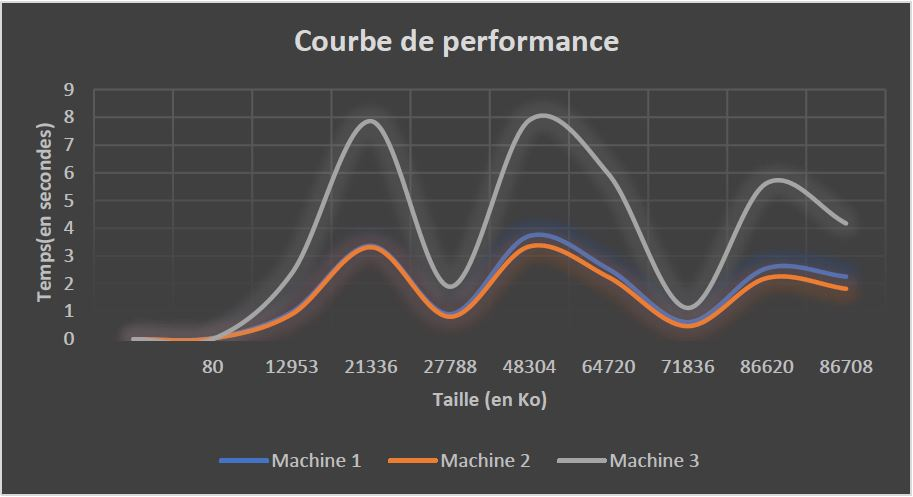
\includegraphics[scale=0.7]{performance_courbe.JPG}
\caption{Courbe de performance}
\label{courbe}
\end{figure}
\paragraph{}
Cette courbe ci-dessus représente le temps d’exécution des fichiers dump testés sur les trois ordinateurs avec des caractéristiques différentes.
\newline
Après une analyse de l'évolution des données, on peut remarquer que la machine 2 est légèrement plus performante en exécution que la machine 1 et vient en dernière position la machine 3.
\newline
Supposons qu'on prenne un fichier dump PA-3772-3828 de taille 27788 ko, l'application va mettre moins de deux secondes pour l’exécuter ce qui correspond relativement aux attentes de Inria-RBA.Par contre sur certains fichiers on peut atteindre jusqu'à sept secondes ce qui diminue la performance de l'application sur une machine peu puissante.


% graphe % ^.



    % * <baptistedecrand@gmail.com> 2018-04-10T13:14:13.026Z:
% Dans cette partie, on doit retrouver la performance de l'application pour afficher un résultat le plus rapidement possible
% on doit pouvoir retrouver la Vitesse d'initialisation, un graphe de la vitesse d'analyse d'un fichier (en fonction de sa taille)
%les resultats attendus par inria pour les fichiers en dessous de 2s




% les complexité des algorithmes
%  les amélioration possible (GPU)
% 2 pages
% PC Batebates
% Système d'exploitation : Windows 10
% Processeur i7 7700HQ 2.80GHz
% GPU Geforce GTX 1050 Nvidia 2Go
% Memoire Ram 8,00 Go
% Disque dur HDD
% PA_608_3464 2.255 s
% PA_1444_1504 2.556 s
% PA_2100_2188 0.615 s
% PA_2244_3156 2.528 s
% PA_2720_1840 3.719 s
% PA_3220_3224 0.905 s
% PA_3548_1148 3.369 s
% PA_3772_3828 0.979 s
% PE_2720_1840 0.042 s
% PE_3548_1148 0.090 s
% 
% PC fixe Thibault
% Système d'exploitation : Windows 10
% Processeur i5 7400 3.00GHz
% GPU Geforce GTX 1060 Nvidia 3Go
% Memoire Ram 16,00 Go
% Disque dur SSHD (hybride ssd, hdd)
%temps en ms :
% PA_608_3464: 1816
% PA_1444_1504: 2203 
% PA_2100_2188: 468
% PA_2244_3156: 2237 
% PA_2720_1840: 3341
% PA_3220_3224: 807
% PA_3548_1148: 3316
% PA_3772_3828: 900
% PE_2720_1840: 25
% PE_3548_1148: 6
% 
% PC portable Thibault
% Système d'exploitation : Windows 10
% Processeur i7 3630QM  2.40 Ghz
% GPU Geforce GT 635M
% Memoire Ram 6,00 Go
% Disque dur HDD (hybride ssd, hdd)
%temps en ms :
% PA_608_3464: 4174
% PA_1444_1504: 5627 
% PA_2100_2188: 1125
% PA_2244_3156: 5954
% PA_2720_1840: 7892
% PA_3220_3224: 1891
% PA_3548_1148: 7860
% PA_3772_3828: 2376
% PE_2720_1840: 0
% PE_3548_1148: 0
% 

%
% Directeur du laboratoire de haute sécurité de Inria-RBA
% Remarques BD:
% ^.


\newpage
\section{Etude des résultats sur la base de données de Inria-RBA}
\subsection{Présentation des données}
\paragraph{}
Comme dit plus haut, Inria-RBA nous a permis l'accès à leur base de données de dumps mémoires pour nos tests, une fois la base d'apprentissage assimilée par le programme.Pour ce test nous sommes partis avec 330 dumps mémoire (fragment de code de logiciel) répartis dans les différentes catégories comme suit :

\paragraph{}
\begin{table}[h]
  \centering
\begin{tabular}{|c|c|}
    \hline
    \rowcolor{gray}
   		Familles & Nombre de fichiers\\
    \hline 
       Bitman&36\\
    \hline 
       Cerber&76\\   
    \hline 
       Deshacop & 1\\       
    \hline
       Fsysna & 1\\
    \hline 
      Gamarue & 1\\
    \hline
      Gpdcode & 1\\
    \hline
      Telsacrypt & 108\\
    \hline
      Xorist & 96\\
    \hline
      Yakes & 1\\
    \hline
      Zerber & 1\\
    \hline
    \rowcolor{blue}
      Goodware & 7\\
    \hline
    \rowcolor{orange}
      Malware & 323\\
    \hline
    
\end{tabular}\\
\caption{Caractéristique de la machine 2}
\label{machine2}
\end{table}

\paragraph{}
Pour bien représenter l'efficacité de notre programme sur cette base de données, nous les représenterons avec le système de "Faux / Vrais" positif ou négatif de cette façon :

\paragraph{}
\begin{table}[h]
\centering
\begin{tabular}{|c|c|c|c|c|}
\hline
Malware & \multicolumn{2}{c|}{Tests positifs} & \multicolumn{2}{c|}{Tests Négatifs} \\
\hline
Absence & 1&14.29\% & 6& 85.71\% \\
\hline
Présence & 323 & 100\% & 0 & 0.00\%  \\
\hline
\end{tabular}
\caption{Statistiques globales pour la métrique Cosine}
\end{table}

\paragraph{}
Note: Par la suite, tout nos exemples d'analyse se feront sur la métrique Cosine, car elle présente les meilleurs résultats globaux en dehors de la métrique Poids que nous détaillerons à part.

\paragraph{}
Pour rappel, nous définissons un "faux positif" comme étant un test désignant une présence qui n'ai pas vraie, un faux négatif, comme étant un test désignant une absence qui n'ai pas vraie. De la même façon avec le vrai positif et négatif. Cette méthode est aussi utilisée pour le diagnostique de maladie, avec un test désignant comme contaminé un patient saint (un faux positif donc).


\paragraph{}
Cette méthode rapportée à notre cas, nous retrouvons dans le tableau ci-dessus 2 grosses colonnes. L'une correspondant au cas où le test effectué est positif, l'autre le test négatif. Comprenez la reconnaissance ou non d'un type de malware selon le tableau. Les deux lignes quant à elles correspondent à la présence effective ou non du malware dans l’échantillon. En somme, les quatre cases correspondant respectivement :

\begin{center}
\begin{tabular}{|c|c|c|c|c|}
  \hline
  faux positif & vrai négatif\\
  \hline
  vrai positif & faux négatif \\
  \hline
\end{tabular}
\end{center}

\paragraph{}
Les cases voisines sont les pourcentages correspondant au taux d'erreur. Notre objectif idéal est donc d'obtenir 100\% de résultats vrais et 0\% d'erreurs :

    % * <baptistedecrand@gmail.com> 2018-04-10T13:14:13.026Z:
% 
% Présentation des test positif/negatif
% Analyse appronfondi des résultats (defaut des métriques et de certaines familles)
% Propositions d'améliorations
% ^. 3 pages
% note Tib : voir pour une comparaison des résultats donnés par inria, voir la correspondance
%				


\begin{figure}[!h] 	
\centering{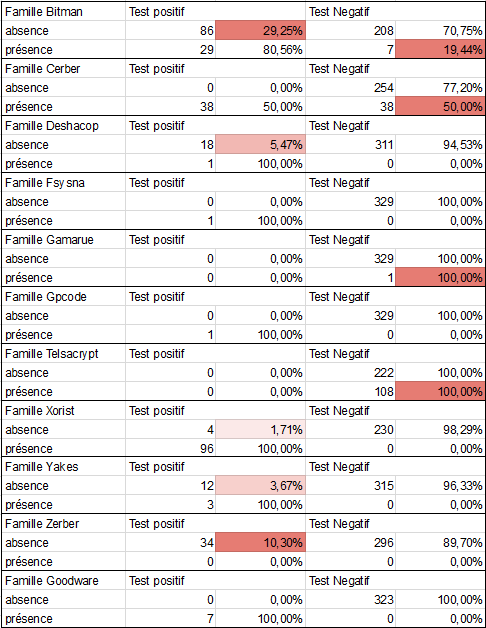
\includegraphics[scale=0.95]{stat-cosine.png}}
    \caption{Exemple de statistiques relevées avec le métrique Cosine}
    \label{mCosine}
\end{figure}




\paragraph{}
Nous pouvons voir sur cet ensemble de données, le taux d’erreur pour un métrique donné. Ici il s'agit de la métrique Cosine que nous avons confronté à l'échantillon présenté plus haut. Pour une lisibilité, les taux d'erreur trop hauts ont été colorisées en rouge, foncé lors que le taux d’erreur est important.


\paragraph{}
Afin de mieux comprendre les liens qu'il pouvait y avoir entre les familles, nous les avons aussi comparées entre elles en utilisant le programme sur leurs bases d'apprentissage. Vous trouverez ci-dessous un tableau représentant la proximité entre les familles de ransomware après ces calculs :


\begin{figure}[!h]
\centering{
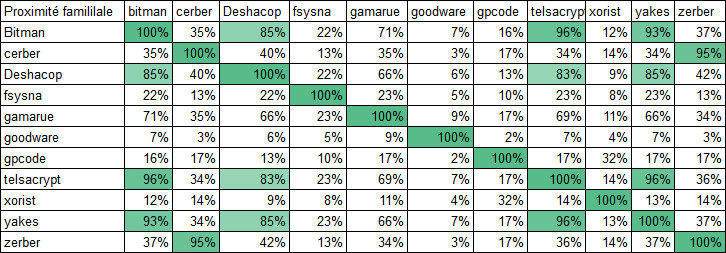
\includegraphics[scale=0.85]{proximiteRansomware.png}}
\caption{Taux de proximité entre les catégories de ransomWare}
\label{proxRansomware}
\end{figure}

\paragraph{}
Comme pour la figure précédente, les taux supérieurs à 70\% de concordance sont colorisés en vert pour un meilleur visuel.

\subsection{Observation des résultats}

La figure~\ref{mCosine} nous montre une fiabilité hétéroclite selon la famille de malware en terme d'efficacité. on observe toutefois de bon résultat globaux sur l’ensemble des familles. Les "100\%" d'erreur chez certaines familles sont à prendre avec des pincettes, un seul dump chez celle-ci a été utilisé dans la base de test connus. 
\\

Avec la figure~\ref{proxRansomware}, on observe que les familles de ransomware ne sont pas si différentes entre elles que ça. On peut les distinguer en plusieurs groupes distincts (pour cela on relève les cellules colorisées en vert d'une même ligne ou colonne) :
\\
	\begin{itemize}
    \item  Bitman - Deshacop - telsacrypt - yakes
    \item  Cerber - zerber
    \end{itemize}
    Et les solitaires :
    \begin{itemize}
    \item Fsysna
    \item Gamarue
    \item goodwares
    \item Xorist
    \end{itemize}
\newpage
\subsection{Analyse des résultats}


\paragraph{}
Maintenant que l'on sait lesquelles métriques sont les plus proches, on sait ceux que le programme aura le plus de mal à différencier. C'est le signe qu'il n'a pas encore été trouvé de signe distinctif au sein du groupe. A la différence de ceux "uniques" qui eux ont une variable spécifique dans leur code. Mais cela permet quand même de faire un premier tri parmi ceux-là.


\paragraph{}
Le jeu des métriques sera de déterminer lequel est le plus adapté. Lorsqu'une catégorie n'est pas déterminée directement, donc quand deux familles ou plus sont confondues par la métrique, il est raisonnable de comparer les groupes suspectés avec une autre métrique, qui sera plus déterministe. Par exemple, il est fort probable que l'ont trouve un dump avec le bon résultat parmi Bitman, Deshacop, Telsacrypt ou Yeakes, mais que l'erreur vienne d'un mauvais choix dans le lot. Et il sera hautement plus compliqué de choisir dans des données plus précises ou un meilleur échantillon.


\paragraph{}
Les résultats mettent en évidence cette nécessité d'aborder le problème avec plusieurs métriques. Car il n'existe pas, à notre connaissance, un algorithme de comparaison qui soit omniscient avec tout les malwares. Nous avons donc choisit de façon un peu arbitraire celui qui présenterai les meilleurs résultats dans nos essais. Comme dit plus haut, il obtient en effet taux de réussite pour la différenciation goodware malware, ce qui est le plus important pour identifier une menace et la neutraliser. C'est pour cette raison que Russel Rao, qui obtient pourtant de meilleurs résultats n'a pas été sélectionné car il confondait à 50\% les goodwares et les malwares. Toutefois, le choix de la métrique reste libre à l'utilisateur.



\subsection{Métrique Poids}
\paragraph{}
Les résultats que l'on a obtenus montrent que l'application est capable de distinguer les ransomwares des goodwares mais qu'elle a du mal à distinguer certaines familles de ransomwares qui ont des vecteurs trop proche.
\paragraph{}
Afin de résoudre ce problème nous avons mis en place une nouvelle métrique que l'on a nommé Poids, qui va permettre de mettre en avant certaines caractéristiques d'une famille.
\paragraph{}
Pour cette nouvelle métrique, chaque composante des vecteurs aura associé une valeur "poids" qui variera entre 0 et 100, cette valeur est établie lors de la construction des vecteurs familiaux et enregistré dans les fichiers de données que charge l'application lors de l'initialisation.
La valeur de base correspond au taux de présence du terme caractéristique dans les dumps mémoires de la famille du ransomware. Ainsi si le terme "sys.dll" est présent dans 58 \% des dumps mémoires correspondant à cette famille, son poids aura une valeur de 58 et lorsqu'un terme est absent il vaut 0. Les vecteurs pour calculer cette distance ne sont pas binaires contrairement aux autres.
\paragraph{}
Le calcul de la métrique Poids se base sur la métrique Cosine car c'est elle qui nous a donné les meilleurs résultats. La distance entre le vecteur sujet (A) et le vecteur familial (B) est calculée de la manière suivante:
\[
    S = \frac{A \cdot B}{||A|| \cdot ||B||}
    \Leftrightarrow S = \frac{\sum_{i=0}^n PoidsA_{i}PoidsB_{i}}{\sqrt{\sum_{i=0}^n PoidsA_{i}}\times\sqrt{\sum_{i=0}^n PoidsB_{i}}}
\]\\


Cette métrique Poids nous donne aussi la possibilité de mieux valorisé certains appels systèmes ou librairies qui sont uniquement présent dans certaines familles. Si on prend par exemple les familles Yakes,Telsacrypt et Bitman qui sont très proches avec environ 95\% de similarité selon la métrique cosine (voir figure~\ref{proxRansomware}). Cependant le vecteur familial de la famille yakes indique que cette famille possède une dizaine de termes caractéristiques que les familles telsacrypt et bitman ne possède pas, en les valorisant c'est-à-dire en augmentant leurs poids initiales, l'application va mieux distinguer un ransomware de type yakes d'un ransoware telsacrypt ou bitman. Sur la métrique simple de cosine, l'application considère que 15 fichiers mémoires sont des Yakes, hors uniquement 3 d’entre eux en sont vraiment. Avec la métrique poids, l'application ne considère plus que quatre fichiers mémoires comme des yakes, dont trois sont vrais, on obtient donc de meilleurs résultats.

La métrique Poids nous a permis de mieux distinguer les ransomwares de type Yakes cependant en appliquant la même méthode aux couples de familles 
telsacrypt-bitman et cerber-zerber, nous n'avons pas constater de meilleurs résultats, ces couples de familles sont très proches cerber et zerber possède très peu de termes caractéristique unique que l'on pourrait valoriser et ces termes ont une très faible présence dans les captures mémoires ( moins de 30\% de taux de présence ). Concernant le couple telsacrypt-bitman, ils n'ont aucun termes caractéristiques unique à mettre en valeur.

\newpage
\section{améliorations possibles}
\paragraph{}
\underline{Virus total}
\todo[inline, color=red!40]{ à ajouter au projet, codé}


\paragraph{}
il existe une application Web dénommée "Virustotal" (https://www.virustotal.com/) autant pour fonction l'analyse de fichier et la détection de logiciel malveillant présents dans le dit fichier. Nous avions pour projet d'intégrer l'API mise à disposition dans notre projet. Cela dans le but d'avoir un résultat comparatif direct et visuel pour l'utilisateur.


\begin{figure}[!h] 	
    \centering{
\includegraphics[scale=0.4]{virustotal_logo.png}}
    \caption{Logo de l'appli web VirusTotal détenu par "Rotarua Limited}
\end{figure}



\paragraph{}
\underline{Meilleure IHM}
\paragraph{}

\paragraph{}
\underline{Développement parallèle}
\paragraph{}

Notre application fonctionne pour un ensemble de fichiers plutôt réduit ( de l'ordre de 500Mo pour la base d'apprentissage). Or pour une base de données réellement efficace il faudrait une source la plus grande, diversifiée et complexe possible.
\paragraph{}
Notre comparaison peut alors prendre du temps avant de s’exécuter correctement, temps qui peut s’avérer décisif pour l'éradication d'une menace. C'est pourquoi le développement parallèle qui utiliserait un processeur graphique réduirait grandement les temps de calcul. On imaginerai donc un groupe d'élément comparé par thread qui tournerait en simultané.

\paragraph{}
En corrélation avec les enseignements de parallélisme suivit ici, nous aurions sans doute utilisé CUDA, pour Compute Unified Device Architecture, développé par Nvidia. Technologie de programmation GPGPU adaptée au processeur graphique Nvidia, le plus courant dans notre groupe.

\begin{figure}[!h] 	
    \centering{
\includegraphics[scale=0.4]{Cuda_logo.jpg}}
    \caption{Logo de Nvidia CUDA, technologie GPGPU}
\end{figure}


\chapter*{Conclusion}
\addcontentsline{toc}{chapter}{Conclusion}
    % * <baptistedecrand@gmail.com> 2018-04-10T13:14:13.026Z:
% La conclusion peut se découper en plusieurs parties:
% -> une reprise du sujet et des objectifs à remplir
%  -> indiquer les objectifs atteint et non atteint
%  -> les difficultés rencontrés au niveau de l'implémentation, de la base de données et au sein de la gestion du groupe
% -> l'état actuel de l'application 
% -> une ouverture
% ^.
Le sujet "analyse forensic de malware" tel qu'on l'a proposé, avait pour but de réaliser un algorithme d'apprentissage supervisé baser sur les chaînes de caractères permettant de détecter les différentes familles de ransomwares grâce à des captures mémoires de programme fourni par l'utilisateur.
\paragraph{}
En amont, on a procédé à l'implémentation des différentes métriques proposé par notre professeur encadrant, ce qui nous a permis de voir la distance entre deux vecteurs, puis à l'extraction des chaînes de caractères présents dans un fichier Dump. En avale, on a attaqué la classification des familles de malwares.
\newline
\`{A} l'aide de ces métriques, les usagers de ce logiciel pourront voir le rapprochement avec les classes de ransomwares. Nous avons réussi à mettre en place les vecteurs familiaux et les vecteurs modèles grâce à la base de données mise à notre disposition par Inria-RBA.
 \paragraph{}
Le projet est plutôt satisfaisant dans son ensemble du moment où on a réussi à faire des recherches nécessaires concernant le sujet et à fournir une documentation qui représente le mémoire du premier semestre.
\newline
Une fois le sujet assimilé, on s'est mis à la partie implémentation du logiciel étape par étape jusqu’à l'aboutissement d'un résultat comme par exemple la détection si un fichier mémoire correspond à un goodware ou pas.
\newline
Parmi les objectifs qu'on s’était fixé au second semestre figurait la possibilité d'augmenter la  quantité  de  famille de ransomware détectable  et chercher à améliorer les dictionnaires vectoriels. Cet objectif est atteint car le programme à ce jour peut reconnaître neuf familles de ransomware. 
\newline

Durant l'implémentation du projet, on a rencontré pas mal de difficulté notamment au calcul des métriques qui donnait de faux résultats sur Hamming, Russel Rao, etc. mais heureusement que c'est résolu.
\newline
\`{A} l'issue de ce projet, nous avons mis en place un outil important permettant d'éradiquer les attaques de ransomware par la simple et bonne raison qu'il nous permet de voir le type de ransomware et une fois identifié, le virus peut être supprimé de l'appareil.


\newpage
\section*{Répartition de la rédaction du mémoire}
\addcontentsline{toc}{section}{Répartition de la rédaction du mémoire}
\begin{table}[!h]
\begin{center}
\begin{tabular}{|l|}
	\rowcolor{gray}
   \hline
   Baptiste Decrand\\
   \hline
   1.1 Construction des vecteurs\\
   \hline
   1.1.1 Vecteur modèle\\
   \hline
   1.1.2 Vecteurs familiaux\\
   \hline
   1.2 Implémentation des métriques\\
   \hline
   1.2.1 Extraction et construction du vecteur sujet\\
   \hline
    1.2.2 Calcul des distances vectoriels\\
   \hline
    2.2.4 Métrique Poids\\
	\rowcolor{gray}
   \hline
   Thanina Alili\\
   \hline
   Introduction\\
   \hline
   1.3 Fonctionnalités\\
	\rowcolor{gray}
    \hline
   Thibault Debonnière\\
   \hline
   2.1.1 Qualité\\
   \hline
   2.2 Etude des résultats sur la base de donnée de Inria-RBA\\
   \hline
   2.3 Améliorations possibles\\
	\rowcolor{gray}
    \hline
   	Ndiasse Thioune\\
    \hline
    2.1.2 Performance\\
   	\hline
   	Conclusion\\
   	\hline
\end{tabular}
\end{center}
\caption{Répartition de la rédaction}
\label{RépartitionRédaction}
\end{table}
\newpage
\chapter*{ANNEXES}
\addcontentsline{toc}{chapter}{ANNEXES}
\newpage


\begin{figure}[!h] 	
    \centering{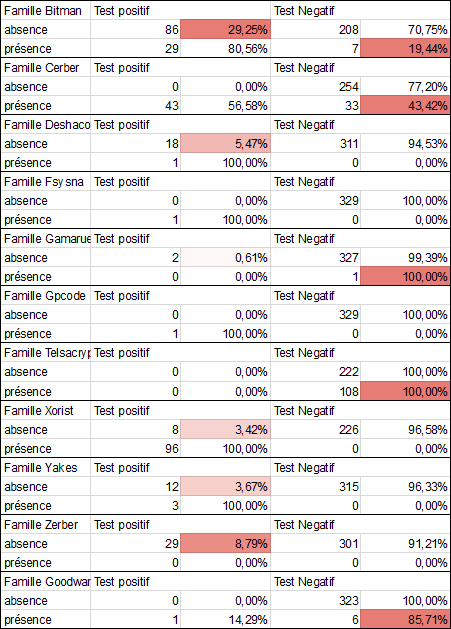
\includegraphics[scale=1.2]{stat-hamming.png}}
    \caption{Données de la métrique HAMMING}
\end{figure}
\newpage
\begin{figure}[!h] 	
    \centering{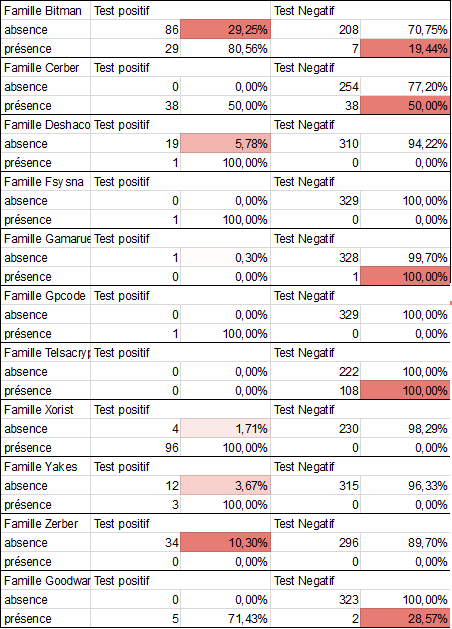
\includegraphics[scale=1.2]{stat-jaccard.png}}
    \caption{Données de la métrique JACCARD}
\end{figure}
\newpage
\begin{figure}[!h] 	
    \centering{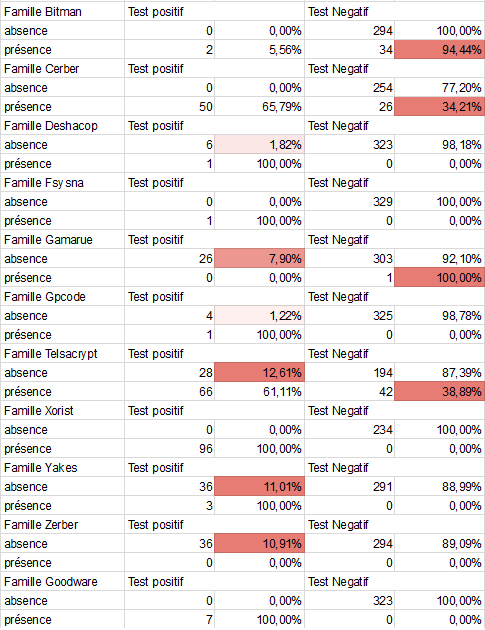
\includegraphics[scale=1.2]{stat-poids.png}}
    \caption{Données de la métrique POIDS}
\end{figure}
\newpage
\begin{figure}[!h] 	
    \centering{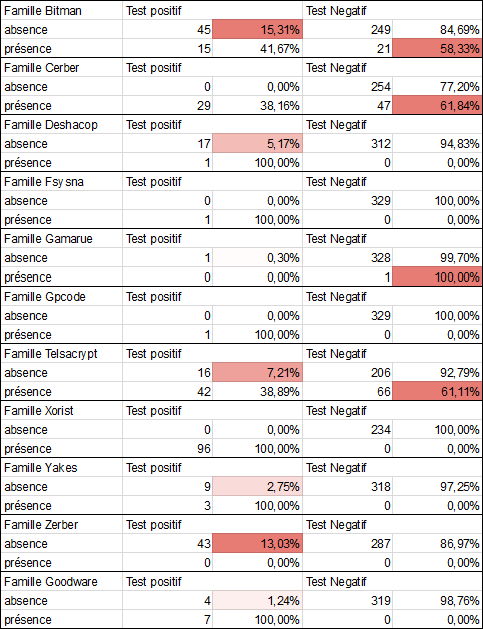
\includegraphics[scale=1.2]{stat-russel.png}}
    \caption{Données de la métrique RUSSEL}
\end{figure}
\newpage
\begin{figure}[!h] 	
    \centering{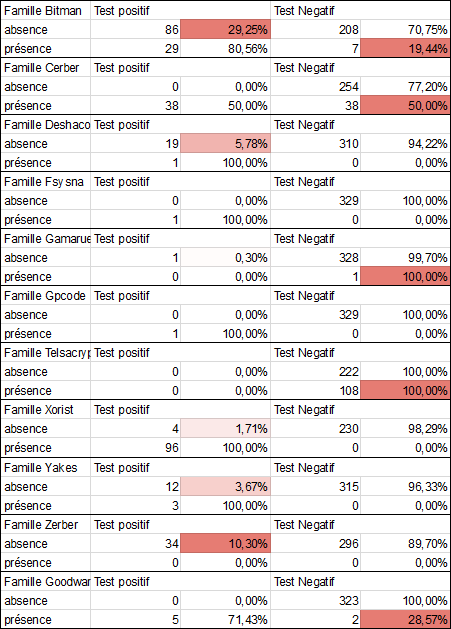
\includegraphics[scale=1.2]{stat-anderberg.png}}
    \caption{Données de la métrique ANDERBERG}
\end{figure}


\begin{thebibliography}{2}
   \bibitem[Document]{lam1}  {\it :A Survey of Binary Similarity and Distance Measures , 2010} 
   \bibitem[Auteur]{cle} Seung-Seok Choi, Sung-Hyuk Cha, Charles C. Tappert - Department of Computer Science, Pace University 
New York, US 

     \bibitem[Document]{lam1}  {\it Properties of Binary Vector Dissimilarity Measures , 2002}  
   \bibitem[Auteur]{cle} Bin Zhang and Sargur N. Srihari - CEDAR,Computer Science and Engineering Department State University of New York
   \bibitem[Document]{lam1}  {\it Comprehensive Survey on Distance/Similarity Measures between Probability Density 
Functions  , 2007} 
   \bibitem[Auteur]{cle} Sung-Hyuk Cha ,INTERNATIONAL JOURNAL OF MATHEMATICAL MODELS AND METHODS IN APPLIED SCIENCES

   \bibitem[Document]{lam1}  {\it Binary-based similarity measures for categorical data and their application in Self-
Organizing Maps  , 2004} 

   \bibitem[Auteur]{cle}Fernando Lourenço , Victor Lobo , and Fernando Bação - Instituto Superior de Estatística e Gestão de Informação, Universidade Nova de Lisboa 

   \bibitem[Document]{lam1}  {\it Experimental analysis of crisp similarity and distance measures, 2004}
    \bibitem[Auteur]{cle}Leila Baccour, Robert I. John - Soft Computing and Pattern Recognition (SoCPaR)

 
\end{thebibliography} 

\end{document}